\documentclass{report}

\usepackage{hyperref}
\usepackage{graphicx}

\author{Manuel Hinz}

\title{Dokumentation des Unipraktikums}

\begin{document}

\maketitle

\tableofcontents
\newpage

\chapter{Einleitung}

\section{Motivation}
Im Moment sind selbstfahrende Autos so ziemlich das technische Thema. Universit\"{a}ten rund um den Globus forschen an verschiedensten Technologien, welche das selbstfahrende Auto braucht. Ein Autohersteller nach dem anderen kauft entweder Startups zu dem Thema auf, oder investiert in eine eigene Forschungsabteilung. Als sich nun die M\"{o}glichkeit eines Praktikums im Rahmen des Elektrotechnikleistungskurses an der Bergischen Universit\"{a}t Wuppertal anbot, fiel die Wahl des Themas leicht. Das dieses Praktikum nicht nur eine gute M\"{o}glichkeit ist um den aktuellen Technischen Entwicklungen nachzueifern, zeigt sich schon an den verschiedenen Aufgaben die zu erledigen sind. Im Laufe des Projektes m\"{u}ssen n\"{a}mlich Motoren mithilfe von H-Br\"{u}cken und Pulsweitenmodulation gesteuert, ein Programm entworfen und ein Raspberrypi in Betrieb genommen werden. Neben dem technischen Wissen, was erlernt und angewendet werden muss (und sich praktischerweise relativ gut mit dem Abiturstoff deckt), wird hier auch ein Einblick in den Universit\"{a}tsalltag erlangt.  
\section{Zielsetzung}
Es gibt viele m\"{o}gliche Aufgaben, die man im Rahmen des Themas l\"{o}sen k\"{o}nnte. Besonders interessant sind hier vor allem das finden von einem und das einparken auf einem Parkplatz, sowie das Teilnehmen am Stra{\ss}enverkehr. Letzteres entf\"{a}llt wegen der Schwierigkeit des Simulierens von anderem Verkehr. Deshalb ist die hier gew\"{a}hlte Aufgabe das finden und befahren einer Parkl\"{u}cke in einem stra{\ss}en\"{a}hnlichen Setting. Genauer gesagt wird das Auto eine Strecke entlangfahren und mit Hilfe von Sensoren eine Parkl\"{u}cke in die es hineinpasst identifizieren und dann dort einparken. Dies wird innerhalb von 16 90-min\"{u}tigen Einheiten \"{u}ber einen Zeitraum von sieben Wochen. Ein weiteres Ziel ist es das f\"{u}r die Vollendung des Projektes n\"{o}tige Wissen f\"{u}r alle Gruppenmitglieder verst\"{a}ndlich zu bearbeiten und die Gruppe damit f\"{u}r das Abitur und weitere Projekte vorzubereiten.

\chapter{Plannung}

\section{Ausblick}

\section{Programmierung}

\subsection{Einleitung}
Bei der Programmierung des Projekts haben wir einen objektorientierten L\"{o}sungsansatz gew\"{a}hlt. Dies haben wir einerseits wegen der Thematisierung der Objekt-Orientierten-Programmierung (OOP) im Informatikunterricht und andererseits wegen dem einfachen Bezug dem man hier zwischen realen Objekten (Sensor, Motor) und zugeh\"{o}rigen Klassen herstellen kann. Au{\ss}erdem ist die OOP einer der Paradigmen, welche in der Realit\"{a}t benutzt werden. 

\subsection{Python}
Als Programmiersprache haben wir Python gew\"{a}hlt, da wir diese Sprache im Informatikunterricht verwenden, sie f\"{u}r Laien leicht verst\"{a}ndlich ist und wir mehrere Personen in der Gruppe bzw. dem nahen Umfeld haben, welche diese Sprache bereits gut k\"{o}nnen. Au{\ss}erdem unterst\"{u}tzt Python die OOP, wodurch die Sprache auch unsere Paradigmenwahl zul\"{a}sst. Da sie eine beliebte und weitverbreitete Sprache ist unterst\"{u}tzt sowohl das aktuelle Image das wir auf dem Pi haben, als auch der Hersteller unsere Sensoren die Sprache. Auch kann man sagen, dass die Sprachwahl es uns erm\"{o}glicht Code, welcher schon fr\"s{u}her von einzelnen Mitgliedern geschrieben wurde, wieder zu benutzen.  Ein Nachteil ist hier, dass Python nicht alle Konzepte der OOP unterst\"{u}tzt (zum Beispiel Abstrakte Klassen, Interfaces/Traits).

\subsection{Programmstruktur}
Jedes gro{\ss}e Bauteil bekommt eine Klasse zugewiesen. Die wichtigen Bauteile sind hier: die Sensoren, die Motoren, die Motortreiber und der Raspberrypi. F\"{u}r die Sensoren haben wir drei Klassen: Einmal eine abstrakte Klasse Sensor, welche definiert, dass jeder Sensor ein Signal auslesen(get\_value) und die Bezeichnung des Pins ausgeben(get\_location) kann. Wir haben dann zwei Klassen, namentlich LightSensor und DistanceSensor, welche von Sensor erben, und jeweils die Methode zum Signalauslesen, sowie den Konstruktor \"{u}berschreiben.

\subsection{Simulation}
Nach dem die Realisierung des praktischen Teils nicht erfolgreich war, wurde die Informatische Leistung auf eine Simulation in Javascript fokussiert, damit wenigstens die Programmierung präsentiert werden kann. Diese Simulation benutz P5.js, was eine Javascriptbibliothek ist. In dieser Simulation soll ein Auto in eine Parklücke, welche durch zwei Hindernisse begrenzt ist, einparken. Es gibt hier momentan eine Klasse für das Auto („Car“) und eine Klasse für die Hindernisse („Obstacle“). Das Hauptskript findet sich in der Datei „sketch.js“. Später würde man auch eine Klasse für die Intelligenz des Autos („Agent“) finden. Im jetzigen Zustand wird die Bewegung des Autos durch einen Geschwindigkeitsvektor und einen Beschleunigungsvektor simuliert. Außerdem wird die Ausrichtung des Autos durch die Ausrichtung des Geschwindigkeitsvektors bestimmt. In der aktuellen Version der Simulation ist der Lenkvorgang beim Einparken verfügbar, sodass für eine erste funktionsfähige Version nur noch Kollisionsdetektion und das Benutzen von Sensoren um Kollisionen zu verhindern fehlt.     
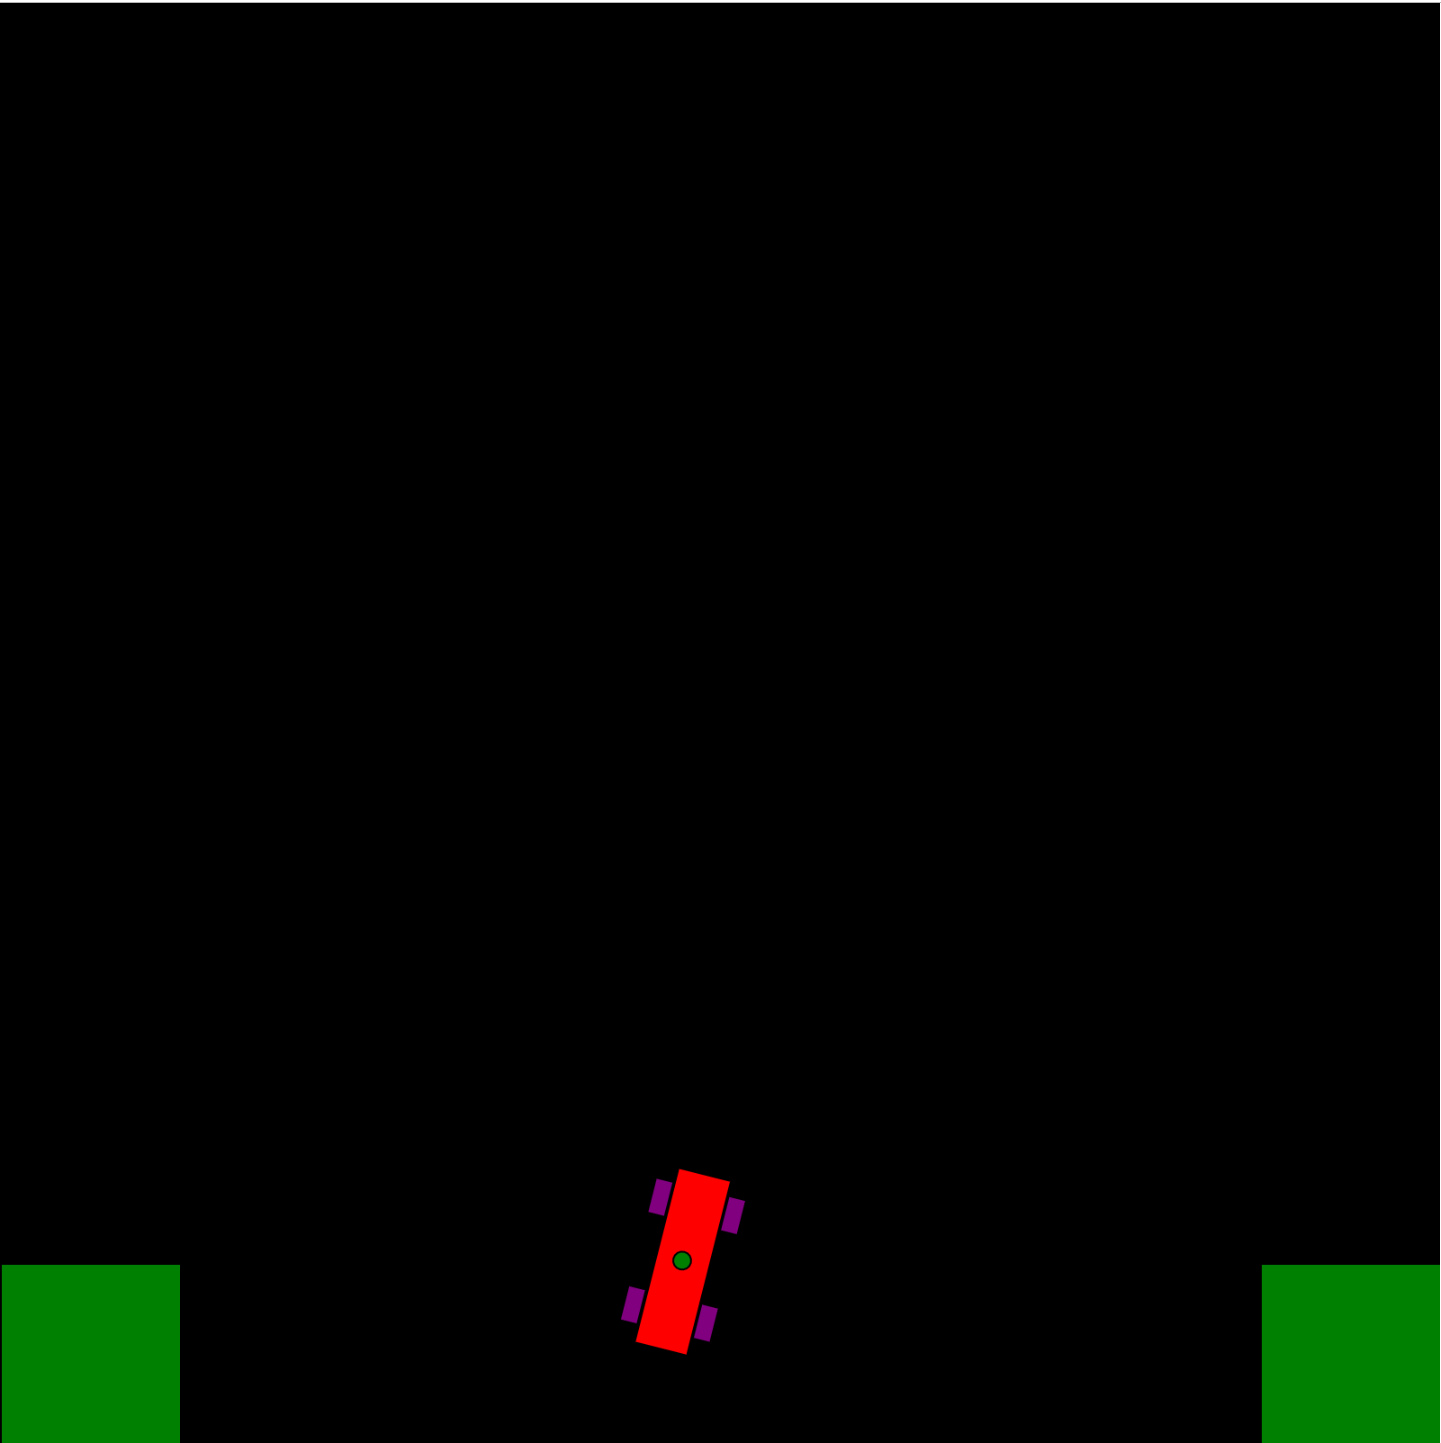
\includegraphics{Bild_Simulation.png}

\subsection{Dateistrukturen}

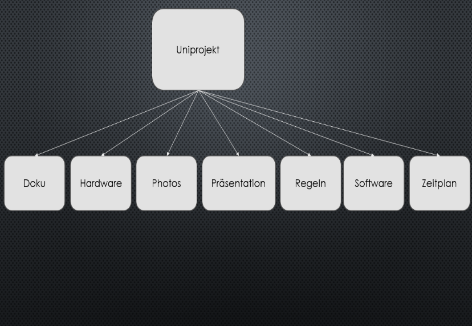
\includegraphics{Struktur.png}
Alle Dateien wurden auf Github hochgeladen. Die Struktur, welche gewählt wurde ist im obigen Bild dargestellt und in diesem Text genauer erläutert. 
Der erste Unterordner trägt den Namen „Doku“. In diesem werden alle Dateien für die Dokumentation gespeichert, der Ordner ist jedoch noch mal in vier Unterordner unterteilt. Diese Ordner sind: erstens „Abgabe“, in welchem alle Dateien für diese Dokumentation zu finden sind, zweitens „Grundwissen“, in welchem Dateien sind, die alle in der Gruppe befähigen sollen, jede Aufgabe eigenständig zu lösen, drittens „Quellen“, in welchem alle unsere Quellen aufgeführt sind und viertens „Tagesdokus“, in welchem alle Tagesdokumentationen sind.
Der zweiter Unterordner „Hardware“ enthält Datenblätter und Messungen in jeweils einem eigenen Unterordner. Es ist hier anzumerken, dass nicht alle Bauteile ein Datenblatt und Messungen haben.
Der Unterordner „Software“ beinhaltet alle eigenen Programme und Skripte. Alle Dateien wurden in die Ordner „Endprogramm“, „Simulation“, „Testen“ und „Tools“ einsortiert. Der Ordner „Endprogramm“ sollte das Programm, was am Ende auf dem Pi läuft, beherbergen. Das wären, im Falle Fertigstellung des Programmes, eine Datei pro Klassengruppe.  Alles was im Unterordner „Simulation“ befindet ist für die Simulation, welche Html und Javascript benutzt. In dem Ordner „Test“ befindet sich Python-Skripte, welche während der Entwicklung des Autos zum Testen einzelner Funktionen (wie z.B. der Reichweite der Abstandssensoren) benutzt werden.
Der Ordner „Regeln“ beinhaltet Dateien, welche Regeln festhalten, die die Zusammenarbeit in der Gruppe erleichtern sollen. Der Ordner Präsentation beinhaltet unterschiedliche Versionen der Präsentation. Im Ordner „Zeitplan“ befindet sich immer der aktuelle Zeitplan samt Anwesenheitsliste.  Alle Fotos sind in dem Ordner „Photos“ um die Dokumentation und die Präsentation zu vervollständigen. 
Durch diese Struktur sollen Dateien immer leicht zu finden sein. Außerdem wird durch diese Struktur die Abgrenzung von einzelnen Aufgabengebieten einfacher, wodurch sich alle Beteiligten leicht in jede Unteraufgabe eindenken können sollen. 


\section{Technologien}

\subsection{Github}

Die Gruppe benutzt Github als unser Versionskontrollsystem. Github bietet sich hier an, weil einerseits git auf dem Raspberrypi ist, wodurch man immer die aktuellste Version des Programmes auf dem Pi haben k\"{o}nnen. Au{\ss}erdem erleichtert Github das gleichzeitige Arbeiten, sodass mehrere Leute gleichzeitig programmieren, und die Programme schlussendlich hochladen k\"{o}nnen. Ein weiteres Plus ist, dass Github eine gro{\ss}e Anzahl an letzten Versionen speichert, wodurch auch sp\"{a}t erkannte Fehler leicht \"{u}berwunden werden k\"{o}nnen. Als letztes Argument f\"{u}r diese Technologie ist zu sagen, dass sie quasi als Dokumentation f\"{u}r alles was auf Github hochgeladen wird dienen kann. Da man jeden Schritt nachvollziehen kann. 

\subsection{Slack}

\subsubsection{Slack-Placeholder}

Slack ist generell eine Kommunikations Software f\"{u}r Unterhaltung. Es k\"{o}nnen Channels er\"{o}ffnet werden die man in unterschiedliche Themen unterteilen kann, je nach Kunde Team oder Projekt. Jeder Benutzer oder jedes Team kann je bei Bedarf verschiedene Channels betreten oder verlassen ganz einfach ohne Komplikationen. Bei jeder neuen Gruppe wir Automatisch ein Bot (KI) erstellt der in das System von Slack einf\"{u}hrt und Befehle oder Abstimmungen etc. in der Gruppe selbst f\"{u}hren/ausf\"{u}hren kann. In Slack kann man auch Audio- und Videochats durchf\"{u}hren f\"{u}r kurze Besprechungen oder Pr\"{a}sentationen.  Wie man die Channels unterteilt ist jeder Gruppe selbst \"{u}berlassen man kann sie f\"{u}r konzentrierte Diskussionen und Informations austausche benutzen oder nur f\"{u}r das Teilen von Dateien jeglichen Typs. Slack hat es geschafft sich mit vielen Tools und Services zu integrieren, dadurch kommen aus abisolierten Posteing\"{a}ngen die Dateien und Nachrichten zu den Team Channels und andersrum. Nat\"{u}rlich ist Slack auch abgesichert, sodass nichts verloren geht und oder was geklaut wird. Die Entwickler arbeiten ganze Zeit an der Sicherheit von Slack damit sie auf dem h\"{o}chsten Niveau ist.

\subsubsection{Benutzung}

Unsere Gruppe benutzte Anfangs Slack f\"{u}r Dateienspeicherung und Kommunikation mittlerweile laden wir auf Slack nur die Tagesdokus hoch und Kommunizieren miteinander, jedoch laden wir die wichtigeren Dateien und generelle Textdokumente auf Github hoch. Da Slack sowie Github als App herunterladbar sind benutzen wir auch diese Mobil, wenn wir unterwegs sind um auf den neusten Stand zu sein. 

\subsection{\LaTeX}

F\"{u}r die Tagesdokumentationen und die Hauptdokumentation wird LaTeX verwendet. Dies ist einerseits eine Referenz auf die echte Welt, in welcher LaTeX oft (im wissenschaftlichem und im privaten) benutzt wird. Andererseits wollen wir von den Vorteilen profitieren. Die Vorteile liegen in darin, dass man einfacher alle Kapitel, Sektionen und Formeln variable gleichzeitig \"{a}ndern k\"{o}nnen. Au{\ss}erdem ist LaTeX eine alternative zu Word, wobei man viele der \"{u}blichen Probleme von Word umgeht. Beispiele w\"{a}ren hier zum Beispiel Verschiebung von Text bei dem Einf\"{u}gen von Bildern, welches man in LaTeX deutlicher definieren muss. 

\subsection{Hilfsprogramm}

Im Rahmen der Dokumentation gab es immer wieder Schwierigkeiten, da man in LaTeX einige Zeichen nicht einfach so schreiben darf, wenn sie entweder nicht von der Kodierung unterstützt werden (Beispiel: ä, Ü) oder schon eine Andere Belegung haben (Bsp.: \_). Damit das schreiben der Dokumentation möglichst schnell passiert wurde deshalb von uns ein Skript geschrieben, welches alle diese problematischen Zeichen durch die LaTeX-Schreibweise ersetzt. Das Skript ist hier jedoch nur eine temporäre Lösung, weshalb man zum Beispiel den Pfad der Latex Datei nicht an das Skript weitergibt, sondern den Pfad innerhalb einer Variablen des Skriptes schreibt.

\section{Elektrotechnik}

\subsection{Grundlagen}

\subsubsection{Umgang mit Elektronik}

\subsubsection{Messen}

\subsubsection{PWM}

\subsubsection{AD/DA Wandler}

\subsubsection{Spannungsteiler}

\subsection{Schaltungen}

\subsection{Messprotokolle}

\subsubsection{H-Br\"{u}cken}
Die Messungen wurden von Murat Mete und Salome Richartz durchgef\"{u}hrt. Genutzt wurden zwei H-Br\"{u}cken, vier Motoren, ein Labornetzger\"{a}t, ein Multimeter, ein Steckbrett und mehrere Leitungen. Damit es uns sp\"{a}ter gelang den Motor anzusteuern, wurde von Pluspol, welcher 9 Volt lieferte, eine externe Leitung gelegt. Daraufhin wurde die H-Br\"{u}cke an die Spannungsversorgung angeschlossen, und diese an einen Motor. Um den Motor anzusteuern haben wir die Leitung, die vorher abgezweigt wurde an einem den zug\"{a}nglichen Pins, der H-Br\"{u}cke, angeschlossen, um ein Signal von einem Microcontroller zu simulieren. Der Strom wurde direkt am Motor gemessen, wo schlie{\ss}lich das Multimeter zum Einsatz kam.

\subsubsection{Motoren}

Die Messungen wurden von Murat Mete und Salome Richartz durchgef\"{u}hrt. Genutzt wurden vier Motoren, ein Labornetzger\"{a}t, ein Multimeter, ein Steckbrett und mehrere Leitungen. Bei diesen Messungen wurde der Stromverbrauch bei Leerlauf und maximale Belastung des Motors festgestellt. Um dies zu erreichen wurde ein Motor nach dem anderen and die Spannungsversorgung angeschlossen. Gemessen wurde direkt am Motor. Um den Leerlauf festzustellen wurde der Motor in die Luft gehoben, somit war dieser nicht belastet. Um den Verbrauch bei maximaler Last zu dokumentieren wurde beim Messen der Motor kurz festgehalten.

\subsubsection{Abstandssensoren}

Die Messungen wurden von Phillip Schulz, Robert Grabarski, Manuel Hinz und Salome Richartz durchgef\"{u}hrt. Genutzt wurden ein Raspberry Pi 3 Model B, Abstandssensoren der Marke GroovePi, ein Schraubenzieher und ein Laptop. Es wurde ein Programm geschrieben, welches eine Nachricht ausgibt, ob der Sensor etwas gefunden hat oder nicht. Der Sensor wurde an den Raspberry Pi angeschlossen und das Programm wurde gestartet. Sobald der der Sensor uns ein “nicht gefunden” zur\"{u}ckgegeben hat, haben wir die Sensibilit\"{a}t des Sensors mithilfe des Schraubenziehers (auf dem Sensor befindet sich ein Potentiometer, welches sich mit dem Schraubenzieher verstellen l\"{a}sst) auf unsere W\"{u}nsche eingestellt.

\subsubsection{Lichtsensoren}

Die Messungen wurden von Phillip Schulz, Robert Grabarski, Manuel Hinz und Salome Richartz durchgef\"{u}hrt. Genutzt wurden ein Raspberry Pi 3 Model B, Lichtsensoren der Marke GroovePi und ein Laptop. Es wurde ein Programm geschrieben, welches uns den gemessenen Helligkeitswert in einem passenden Format zur\"{u}ckgibt. Der Sensor wurde unterschiedlichen Helligkeitssituationen ausgesetzt und die Werte verglichen.


\chapter{Realisierung}

\section{Probleme}

\subsection{Gel\"{o}ste Probleme}

\subsection{Ungel\"{o}ste Probleme}

\section{Teamdynamik}

Am Anfang ergab sich die Problematik, da unsere Gruppe nur aus fünf Individuen bestand, dass wir keinen Teamleiter ernennen konnten. Darum hat sich die Gruppe entschlossen, einzelne Teilverantwortliche zu ernennen. Diese waren für einen bestimmten Bereich verantwortlich, mussten jedoch diesen nicht alleine bearbeiten, denn sie waren dazu befähigt ein anderes Teammitglied, welches zu diesem Zeitpunkt keine Arbeit hatte oder einen Leerlauf, für bestimmte Aufgaben heranzuziehen.
Somit ergab sich eine stetige Kommunikation innerhalb der Gruppe, den trotz der Hauptverantwortung des einzelnen musste dieser nicht ein Experte in diesem Bereich sein, mithilfe des Informationsaustausches.
Es ergaben sich jedoch auch einige Probleme durch diese Art der Aufgabenverteilung. Ein Mitglied der Gruppe war Aufgrund einer Krankheit die ersten 4 Termine nicht anwesend und musste innerhalb eines Termines auf den aktuellen Stand des Projektes gebracht werden. Dies konnte man jedoch nicht verhindern. Ein anderes Problem war die schwindende oder keinerlei vorhandene Motivation einzelner Individuen, die jedoch für schwerwiegende Bereiche verantwortlich waren, darüber hinaus arbeiteten diese auch nur wenn man sie explizit auf bestimmte Aufgaben ansetzte. 
Diese Probleme hätte man lösen können indem man mehrere für einzelne Bereiche Verantwortlich hätte machen sollen oder einen Hauptverantwortlichen für das komplette Projekt erklären können.
Die Allgemeine Dynamik des Teams war rückblickend positiv. Jeder hat seinen Teil für das Projekt beigetragen und anderen Mitgliedern geholfen.


\chapter{Anhang}

\section{Quellen}

\subsection{Elektrotechnik}
\begin{itemize}

\item \url{http://cdn-reichelt.de/documents/datenblatt/A100/BC546_48-CDIL.pdf}


\item \url{http://anleitung.joy-it.net/wp-content/uploads/2017/06/SBC-MotoDriver2-Anleitung.pdf}

\item \url{http://cdn-reichelt.de/documents/datenblatt/A300/COM_MOTOR_RAD_DB-DE.pdf}

\end{itemize}

\subsection{RaspberryPi}

\begin{itemize}

\item \url{https://www.terraelectronica.ru/pdf/show?pdf_file=%252Fds%252Fpdf%252FT%252FTechicRP3.pdf}

\item \url{http://www.netzmafia.de/skripten/hardware/RasPi/RasPi_GPIO_C.html}

\item \url{https://help.github.com/enterprise/2.14/user/articles/generating-a-new-ssh-key-and-adding-it-to-the-ssh-agent/}

\item \url{https://devmarketer.io/learn/set-ssh-key-github/}

\end{itemize}

\subsection{GrovePi}

\begin{itemize}

\item \url{http://cdn-reichelt.de/documents/datenblatt/A300/GRV_IR_DISTANCE_AL-EN.pdf}

\item \url{http://www.mouser.com/catalog/specsheets/Seeed_101020022.pdf}

\item \url{https://github.com/DexterInd/GrovePi/blob/master/Hardware/GrovePi%2B%20v3.0.pdf}

\item \url{https://github.com/DexterInd/GrovePi/blob/master/Hardware/GrovePi%20Graphical%20Datasheet.jpg}

\end{itemize}

\end{document}